\chapter{Fehlerrechnung und Auswertungen im Praktikum} \label{v:fehler}

Dieses Kapitel ist aus dem Skript des Grundpraktikums für Physiker übernommen. Der Inhalt sollte derselbe sein, wie in Kapitel \ref{v:fehlerJW}, die Formulierungen sind aber etwas präziser und mathematischer gehalten.\\
Wenn Sie mit dem vorherigen Kapitel zur Fehlerrechnung nichts anfangen konnten, schauen Sie sich doch alternativ mal dieses hier an.

\section{Allgemeines}

Dieser Abschnitt m"usste eigentlich richtiger hei"sen: "`Rechnen mit
Ungenauigkeiten"'\index{Ungenauigkeiten}. Im Folgenden sollen kurz
einige Grundlagen zur Fehlerrechnung\index{Fehlerrechnung},
Statistik\index{Statistik} und Auswertung von
Messdaten\index{Auswertung} dargelegt werden, soweit sie f"ur
dieses Praktikum wichtig sind. F"ur eine genauere Betrachtung sei
auf die Spezialliteratur
%\cite{beving,bron,npp,kamke,physmess,lichten,tbstat,tbnum,taylor,messunsicher}
verwiesen.\\

\noindent
Dieser Abschnitt ist der Praktikumsanleitung für Physiker entnommen. Inhaltlich sollte er größtenteils mit dem vorherigen Abschnitt übereinstimmen, führt aber einige der Konzepte in größerer Tiefe ein.

\section{Vorbemerkung}

Eine physikalische Gr"o"se\index{Gr"o"se!Physikalische} kennzeichnet
Eigenschaften und beschreibt Zust"ande sowie Zustands"anderungen von
Objekten der Umwelt. Sie muss nach einer Forderung von
\person{Einstein} messbar sein. Die Vereinbarung, nach der die
beobachtete physikalische Einheit quantifiziert wird, ist die
Einheit der physikalischen Gr"o"se. Somit besteht eine physikalische
Gr"o"se {\bf G} immer aus einer quantitativen Aussage G (Zahlenwert)
und einer qualitativen Aussage [G] (Einheit): {\bf G} = G $\cdot$
[G].

F"ur physikalische Gr"o"sen gilt: "`Physikalische Gr"o"se = Zahlenwert
$\cdot$ Einheit"', also bitte immer Einheiten angeben.\footnote{Die
Betreuerinnen sollen Protokolle mit fehlenden Einheiten
zur"uckgeben.} Gesetzlich vorgeschrieben ist die Verwendung des
\emph{Internationalen Einheitensystems
(SI-Einheiten)}\index{SI-Einheiten}. Im amtlichen und gesch"aftlichen
Verkehr d"urfen nur noch SI-Einheiten\index{Einheit} benutzt werden. Teilweise muss man als Naturwissenschaftler aber
auch mit anderen, "alteren Einheiten umgehen k"onnen (Bsp.: Torr,
Gau"s). %Einen sehr sch"onen "Ubersichtsartikel "uber physikalische
%Gr"o"sen, deren Nomenklatur und Einheiten, finden Sie in Ref.~\cite{codata}.

Die Messung einer physikalischen Gr"o"se\index{Gr"o"se!physikalische}
erfolgt %durch Vergleich der Einheit dieser Gr"o"se nach der
Messmethode der (SI-)Vereinbarung oder einem darauf aufbauenden
Messverfahren. Je nach Genauigkeit des Messverfahrens tritt ein
unterschiedlich grosser Messfehler (Ungenauigkeit, Abweichung) auf.
Dabei ist zwischen den \emph{systematischen}, f"ur das Messverfahren
charakteristischen Messfehlern\index{Messfehler} und den
\emph{zuf"alligen} oder \emph{statistischen}, vom einzelnen
Experiment abh"angigen Fehlern zu unterscheiden. Zu systematischen
Messfehlern geh"oren z.B. eine falsche Kalibrierung eines
Messger"ates, Ablesefehler (Parallaxe), falsche Justierung,
Messwertdrift, etc. Zu statistischen Fehlern geh"oren (zuf"allige)
Schwankungen wie elektronische Triggerschwankungen,
Temperaturschwankunken, Rauschen, ungenaues Anlegen von Ma"sst"aben
etc. Zur grafischen Analyse der Messwertschwankungen dient das
Histogramm. Bei zuf"alligen Messfehlern ist die H"aufigkeitsverteilung
der Messwerte $N_j(x_j)$ symmetrisch zu einem Mittelwert, dem
Erwartungswert $\mu$. Wird die Anzahl $n$ der Wiederholungsmessungen
stark erh"oht, so geht die (diskrete) relative H"aufigkeitsverteilung
$N_j(x_j) \rightarrow h(x)$ in eine glockenf"ormige Normalverteilung
(\person{Gau"s}sche Verteilungsfunktion) mit der
Halbwertsbreite\index{Halbwertsbreite} $\Gamma$ (= halbe Breite der Kurve
in halber H"ohe des Maximums, engl.~\textsc{HWHM=Half Width at Half
Maximum}) der Messwerte "uber:
%
\begin{important}
\begin{equation}\label{e:gaussnormal}
    h(x) = \frac{1}{\sqrt{2 \pi}\sigma} e^{-\frac{(x-\mu)^2}{2 \sigma^2}}
    \qquad \mbox{mit} \qquad
    \sigma = \frac{\Gamma}{\sqrt{2 \, \ln 2}} \, .
\end{equation}
\end{important}

Der Parameter $\sigma$ ist ein Ma"s f"ur die Breite der
Verteilungsfunktion $h(x)$: 68,3~\% der Messwerte liegen im Bereich
$\mu - \sigma < x < \mu + \sigma $. Aus der H"aufigkeitsverteilung $h(x_j)$
einer endlichen Anzahl $N$ von Messungen der $m$ diskreten
Messwerte $x_1, \ldots x_m$ lassen sich f"ur 
$\mu$ und $\sigma$ nach der Theorie der
Beobachtungsfehler von \person{Gau"s} Sch"atzwerte berechnen.
Demnach ist die beste N"aherung f"ur $\mu$ der arithmetische
Mittelwert $\bar{x}$, f"ur $\sigma$ die
Standardabweichung $s$, die sich aus der
Fehlersumme berechnet (s.u.). 
%Letztere ist minimal, wenn der
%arithmetische Mittelwert als Erwartungswert gesetzt wird (siehe
%unten).

\section{Ungenauigkeiten und Fehler}

Alle Messvorg"ange liefern Messergebnisse mit einem Fehler, der
nach einer verbindlichen "Ubereinkunft ein Ma"s f"ur die Genauigkeit
des Messergebnisses darstellt. Ein Beispiel: Die L"ange eines
Stabes wird durch Anlegen eines Ma"sstabes bestimmt. Dann sind zwei
Arten von Fehlern m"oglich:
%
\begin{enumerate}
  \item der systematische Fehler des Ma"sstabs, der sich durch genauen Vergleich
   mit dem Urmeter\index{Urmeter} ermitteln l"asst,
  \item der zuf"allige Fehler, der sich durch Unsicherheiten beim Anlegen des
 Ma"sstabs ergibt.
\end{enumerate}

Alle Messergebnisse m"ussen deshalb mit Fehlerangabe $\bar{x} \pm
\Delta x$ angeben werden. In den meisten
F"allen darf man annehmen, dass die Messwerte um den wahren Wert
statistisch streuen, d.h. dass die Abweichungen im Betrag
schwanken und im Mittel gleich oft positiv wie negativ
ausschlagen. Dann ist der beste Wert (Bestwert)\index{Bestwert},
den man aufgrund von $n$ wiederholten Messungen mit Messergebnis
$x_i$ angeben kann, der Mittelwert\index{Mittelwert} $\bar{x}$:
%
\begin{important}
\begin{equation}\label{e:mw}
\mbox{Mittelwert: } \,  \bar{x} = \frac{1}{n} \sum_{i=1}^n x_i \,
.
\end{equation}
\end{important}
%
Au"ser den Streufehlern, die man auch zuf"allige - oder statistische
- Fehler nennt, treten gew"ohnlich auch so genannte systematische
Fehler auf. Ist ein Messger"at falsch kalibriert, wird es zum
Beispiel immer zu gro"se Werte liefern. Um eine Aussage "uber die
Zuverl"assigkeit des Messergebnisses machen zu k"onnen, muss die
Gr"o"se dieser beiden Fehlereinfl"usse abgesch"atzt werden. Die
Aufgabe der Fehlerrechnung ist also die Bestimmung des Fehlers
$\Delta x = \Delta x_{\rm syst.} + \Delta x_{\rm stat.}$. Das Ergebnis der
Messung mit Fehlerangabe\index{Fehlerangabe} lautet dann:
%
\begin{equation}\label{e:ergfehler}
  \mbox{Ergebnis mit Fehlerangabe: } \,  \bar{x} \pm \Delta x \, .
\end{equation}
%
Diese Angabe bedeutet: Man erwartet, dass der wahre Wert $x_w$ im
Bereich $\bar{x} - \Delta x \leq x_w \leq \bar{x} + \Delta x $
liegt. $\Delta x$ nennt man den absoluten Fehler. Es kann auch der
relative Fehler angegeben werden: $\Delta x / \bar{x}$.

Da jede gemessene physikalische Gr"o"se mit einem Fehler behaftet ist,
macht es keinen Sinn als Ergebnis eine Zahl mit vielen Ziffern
anzugeben. Die Zahl der angegebenen Ziffern sollte an die Gr"o"se des
Fehlers angeglichen werden, d.h. das Ergebnis ist entsprechend
sinnvoll zu runden. Das Ergebnis und der Fehler werden an der
gleichen Stelle gerundet. Der Fehler wird normal gerundet.


\section{Systematische Fehler}

Systematische Fehler\index{Fehler!systematische} bei Messungen im
Praktikum r"uhren haupts"achlich von Ungenauigkeiten der Messger"ate
oder der Messverfahren her. Abweichungen der Messbedingungen, wie
z.B. der Temperatur, spielen in der Regel eine untergeordnete
Rolle. Beispiele f"ur systematische Fehler sind:
%
\begin{itemize}
  \item Eine Stoppuhr geht stets vor oder nach
  \item Ein Voltmeter zeigt wegen eines Kalibrierfehlers einen stets zu gro"sen
   (oder zu kleinen) Wert an
  \item Der Ohmsche Widerstand in einer Schaltung weicht vom
  angegebenen Nominalwert ab.
  \item Eine Beeinflussung der Messung durch Messger"ate (z.B.
  Innenwiderst"ande) wird nicht ber"ucksichtigt.
\end{itemize}
%
Systematische Fehler haben stets einen festen Betrag und ein
eindeutiges Vorzeichen. Sie "andern sich auch nicht, wenn die Messung
mit der gleichen Anordnung und den gleichen Ger"aten wiederholt wird.
Da das Vorzeichen nicht bekannt ist, muss man sie auch mit dem
unbestimmten Vorzeichen $\pm$ angeben. F"ur die Absch"atzung des
Betrages gelten die folgenden Hinweise.

F"ur Messger"ate sind die maximal erlaubten Abweichungen $\Delta
x_{\rm syst.}$ einer Anzeige $x$ vom wahren Wert in der Regel durch
Herstellungsnormen festgelegt (G"ute des Ger"ates, siehe
Beschreibung bei "`Messger"aten"'). F"ur elektrische Messger"ate ist
der Begriff "`G"uteklasse"' eingef"uhrt worden. Diese gibt den
erlaubten systematischen Fehler als Prozentwert vom Vollausschlag
an. Diesen Fehler setzt man dann f"ur alle Messungen in diesem
Messbereich an.

Bei L"angenmessger"aten betr"agt der m"ogliche systematische Fehler
selten mehr als wenige Promille vom Messwert und kann daher
gegen"uber den Streufehlern in den meisten F"allen vernachl"assigt
werden. F"ur eine quantitative Absch"atzung kann die folgende Formel
verwendet werden:
%
\begin{equation}\label{e:skalafehler}
  \frac{\Delta x_{\rm syst}}{x} =
  \frac{\mbox{1 Skalenteil der Skala}}{\mbox{Skalenteile bei Vollausschlag.}}
\end{equation}

Stoppuhren sind noch genauer und Ihr Fehler kann zu $\Delta
x_{\rm syst} = \mbox{kleinster Skalenwert} + {\rm 0.005} \cdot
\mbox{Messwert} $ abgesch"atzt werden.

Bei der Messung von Temperaturen mit einem Fl"ussigkeitsthermometer
betr"agt der Ger"atefehler etwa 1~Strichabstand.


\section{Statistische, zuf"allige Fehler}

Ursachen f"ur zuf"allige Fehler\index{Fehler!statistische} sind z.B.
Schwankungen der Messbedingungen w"ahrend der Messung oder auch
Ungenauigkeiten bei der Ablesung von Messinstrumenten (z.B.
Parallaxe). Um den Betrag des Streufehlers absch"atzen zu k"onnen,
wiederholt man die Messung mehrfach. Ein Ma"s f"ur die Streuung kann
dann aus den Abweichungen $x_i - \bar{x}$ der einzelnen Messwerte
vom Mittelwert gewonnen werden, die von Gau"s als
Standardabweichung $s$ f"ur $n$ Messungen $x_i$ definiert wurde:
%
\begin{equation}\label{e:standabw}
  s = \sqrt{ \frac{1}{n-1} \sum_{i=1}^n \left( x_i - \bar{x} \right)^2 }
\end{equation}

Die Standardabweichung $s$ repr"asentiert die Genauigkeit der
einzelnen Messung und damit auch des Messverfahrens. Deshalb wird
$s$ auch als mittlerer quadratischer Fehler der Einzelmessung
bezeichnet. Je mehr Einzelmessungen vorliegen, umso genauer wird
der Mittelwert sein. Der mittlere quadratische Fehler des
Mittelwertes $\Delta x_{\rm stat.}$ ist nach der Fehlertheorie um den
Faktor $\nicefrac{1}{\sqrt{n}}$ kleiner.
%
\begin{important}
\begin{equation}\label{e:fmw}
 \Delta x_{\rm stat} = \frac{s}{\sqrt{n}}
     = \sqrt{ \frac{1}{n(n-1)} \sum_{i=1}^n \left( x_i - \bar{x} \right)^2 }
\end{equation}
\end{important}
%
Dieser Wert $\Delta x_{\rm stat}$ wird manchmal in Anlehnung an
die Normalverteilung als $\sigma_{\bar{x}}$ bezeichnet. 
Dabei sollte der Wert $\sigma_{\bar{x}}$, der den Fehler auf
den arithmetischen Mittelwert $\bar{x}$ angibt, {\it nicht} mit dem
Fehler $\sigma=s$ der Einzelmessung $x_i$ verwechselt werden!
Die Fehlerrechnung
erlaubt dann die Aussage (wenn systematische Fehler wesentlich
kleiner sind), dass der wahre Wert mit einer Wahrscheinlichkeit
von 68\% im Intervall mit der Breite $\sigma_{\bar{x}}$ um den Mittelwert
liegt: $\bar{x} - \sigma_{\bar{x}} < x_w < \bar{x} + \sigma_{\bar{x}} $.

%Nach der Theorie der Beobachtungsfehler (t-Verteilung nach
%Student, alias \person{W. S. Gosset}) sind bei normalverteilten
%Messgr"ossen die Vertrauensgrenzen abh"angig von der Anzahl $n$ der
%Messungen und der Standardabweichung $s$ des Messverfahrens:
%
%\begin{equation}\label{e:t-vert}
%    x = \bar{x} \pm t_P \cdot \frac{s}{\sqrt{n}}
%\end{equation}
%
%Der Faktor $t_P$ folgt aus der Student-t-Verteilung und ist
%abh"angig von der Anzahl der Wiederholungsmessungen und der
%geforderten statistischen Sicherheit $P$
%\cite{bron,tbstat}. F"ur gro"se $n$ entspricht
%$t_{\numprint[\%]{68.3}}$=1. %, d.h. $\Delta x = \Delta \bar{x}$.
%Einige Werte f"ur $t_P$ sind in Tabelle~\ref{t:student} aufgef"uhrt.

Im Praktikum, wie meistens in der
Physik, k"onnen wir uns mit 1$\sigma$, also 68,3~\% Sicherheit zufrieden geben.
Bitte geben Sie Ihre Ergebnisse in den Protokollen auch so an,
d.h. benutzen Sie die $1\sigma$"=Regel f"ur Ihre Fehlerangaben.
Liegt neben der statistischen Unsicherheit auch noch ein
systematischer Fehler vor, so ist als Gesamt-Messfehler die quadratische Summe
der beiden Fehler anzugeben.
%
%\begin{table}[htb]%
%  \centering%
%  \caption[Student-Verteilung: Werte von $t_P$]{\label{t:student}Einige Werte
%  von $t_P$ bei der Student"=t"=Verteilung
%   f"ur die angegebene statistische Sicherheit.}%
%  \begin{tabular}{rrrr}%
%    \toprule
%    $n$ & 68.3\% & 95\% & 99.7\% \\ \midrule
%    3   & 1.32 & 4.3 & 19.2 \\
%    5   & 1.15 & 2.8 & 6.6\\
%    10  & 1.06 & 2.3 & 4.1\\
%    100 & 1.00 & 2.0 & 3.1\\ \bottomrule
%  \end{tabular}
%\end{table}


\section{Gewichteter Mittelwert}

Bei Vorliegen mehrerer \emph{unabh"angiger} Ergebnisse ist es "ublich,
den gewichteten Mittelwert\index{Mittelwert!gewichtet} anzugeben:
%
\begin{important}
\begin{equation}\label{e:gewmittel1}
 \bar x = \frac{
   \sum\limits_i \frac{x_i}{\sigma_i^2 }
    }{
    \sum\limits_i \frac{1}{\sigma_i^2}
    }
    \quad \mbox{mit Fehler: } \quad
    \sigma  = \sqrt{\frac{1}{\sum\limits_i \frac{1}{\sigma_i^2}} } \, .
\end{equation}
\end{important}
%
Bei stark unterschiedlich genauen Werten greift man besser auf
folgende Berechnung des Fehlers zur"uck:
%
\begin{equation}\label{e:gewsigma2}
 \sigma  = \sqrt {\frac{{\sum {\frac{{\left( {x_i  - \bar x}
 \right)^2 }}{{\sigma _i^2 }}} }}{{\left( {n - 1} \right)\sum
 {\frac{1}{{\sigma _i^2 }}} }}} \, ,
\end{equation}
%
oder nimmt das Maximum des mit den beiden obigen Formeln
berechneten Fehlers.

\section{Lineare Regression}

Hat man die Messwerte $y_i(x_i)$ vorliegen und vermutet einen
linearen Zusammenhang $y=m\cdot x + b$, so kann man dies einfach
mit der linearen Regression\index{Lineare Regression} testen. 

\subsection{Einfache Regression}

Ohne Ber"ucksichtigung bzw.~Kenntnis der Fehler auf die Messwerte 
$y_i$ ergibt sich f"ur die Steigung aus der linearen Regression:
%
\begin{equation}
m = \frac{{n\sum {x_i y_i  - \sum {x_i \sum {y_i } } } }}{{n\sum
{x_i^2  - \left( {\sum {x_i } } \right)^2 } }}
\end{equation}
%
und der Achsenabschnitt ist
%
\begin{equation}
b = \frac{{\sum {x_i^2 \sum {y_i }  - \sum {x_i \sum {x_i y_i } }
} }}{{n\sum {x_i^2  - \left( {\sum {x_i } } \right)^2 } }}
\end{equation}
%
Die jeweiligen Fehler berechnen sich zu:
%
\begin{equation}
\sigma_m^2  = \frac{{n\sum {\left( {y_i  - b - mx_i } \right)^2 }
}}{{\left( {n - 2} \right)\left( {n\sum {x_i^2  - \left( {\sum
{x_i } } \right)^2 } } \right)}}
\end{equation}
%
\begin{equation}
\sigma_b^2  = \frac{{\sum {x_i^2  \cdot } \sum {\left( {y_i  - b -
mx_i } \right)^2 } }}{{\left( {n - 2} \right)\left( {n\sum {x_i^2
- \left( {\sum {x_i } } \right)^2 } } \right)}}
\end{equation}
%
und der Korrelationskoeffizient\index{Korrelationskoeffizient}
berechnet sich folgenderma"sen:
%
\begin{equation}
 r = \frac{
 {n\sum {x_i y_i  - \sum {x_i \sum {y_i } } } }
 }
 {
 {\sqrt{n\sum {x_i^2  - \left( {\sum {x_i } } \right)^2 }} \cdot
  \sqrt{n\sum {y_i^2  - \left( {\sum {y_i } } \right)^2 } } }
 }
\end{equation}
%
Mathematisch liefert der Korrelationskoeffizient ein Ma{\ss} daf"ur, ob die Annahme eines linearen Zusammenhangs zwischen den $x_i$ und $y_i$ sinnvoll ist. Je dichter der Betrag des Korrelationskoeffizienten bei Eins liegt, desto besser ist die Linearit"at.\\
Man sei aber vorsichtig, aus einem guten $r$ sofort auf einen
wirklich physikalischen linearen Zusammenhang zu schlie"sen.

\subsection{Regression mit Messfehlern} \label{v:LinRegErr}

Unter der Voraussetzung, dass nur die
$y_i$-Werte mit dem Fehler $\sigma_i$ fehlerbehaftet, w"ahrend die
$x_i$-Werte fehlerfrei sind, ergibt sich f"ur die lineare Regression:
\begin{align*}
\Delta&=\sum{\frac{1}{\sigma_i^2}}\sum{\frac{x_i^2}{\sigma_i^2}}-
\left(\sum{\frac{x_i}{\sigma_i^2}}\right)^2 & &
\\
%
m&=\frac{1}{\Delta}\left(\sum{\frac{1}{\sigma_i^2}}
\sum{\frac{x_iy_i}{\sigma_i^2}}-\sum{\frac{x_i}{\sigma_i^2}}\sum{\frac{y_i}{\sigma_i^2}}
\right)
&\sigma_m&=\sqrt{\frac{1}{\Delta}\sum{\frac{1}{\sigma_i^2}}} \\
%
b&=\frac{1}{\Delta}\left(\sum{\frac{x_i^2}{\sigma_i^2}}
\sum{\frac{y_i}{\sigma_i^2}}-\sum{\frac{x_i}{\sigma_i^2}}\sum{\frac{x_iy_i}{\sigma_i^2}}
\right) \hspace{11mm}
&\sigma_b&=\sqrt{\frac{1}{\Delta}\sum{\frac{x_i^2}{\sigma_i^2}}} \\
%
\chi^2&=\sum{\left[\frac{1}{\sigma_i}\left(y_i-mx_i-b\right)\right]^2} & &
\end{align*}


\section{Mathematische Behandlung}

\subsection{Grundlagen der Fehlerrechnung: Bestwert und Fehler}

Wir betrachten im Folgenden einen vorher berechneten Mittelwert
aus Messergebnissen f"ur eine physikalische Gr"o"se und bezeichnen
diesen mit $M$. F"ur diese Gr"o"se $M$ kennen wir den wahren Wert
$M_W$, der in einem wirklichen Experiment nat"urlich unbekannt ist,
aber als existent angenommen werden kann. Jeder Messwert $M_i$ der
Gr"o"se $M$ weicht vom wahren Wert um den absoluten Fehler $\Delta M_i$
ab:
%
\begin{equation} \label{b}
 \Delta M_i = M_i - M_W \, .
\end{equation}
%
Das Endergebnis einer $n$-mal wiederholten Bestimmung von $M$ soll
durch einen Bestwert $M_B$ beschrieben werden, der der Vorschrift
%
\begin{equation} \label{c}
\sum_{i=1}^{n}\, (M_{i} - M_{B})^{2} = f(M_{B}) = \mbox{Minimum}
\end{equation}
%
gen"ugt, die als \person{Gau"s}sche Methode der kleinsten
(Fehler-)Quadrate zur Bestimmung des Bestwertes\index{Bestwert}
bezeichnet wird. F"uhrt man die Bestimmung des Minimums nach der
Vorschrift
%
\begin{equation} \label{d}
 \frac{d}{d M_B} \sum_{i=1}^{n}(M_{i} - M_{B})^{2} = 0
\end{equation}
%
aus, so ergibt sich
%
\begin{equation} \label{e}
 M_{B} = \frac{1}{n} \sum_{i=1}^{n} M_{i} = \bar M
\end{equation}
%
und damit die Definition:
%
\begin{definition} \label{def:bestwert}
  Der Bestwert ist gleich dem arithmetischen Mittel.
\end{definition}

Der in (\ref{b}) definierte absolute Fehler der
Einzelmessung\index{Fehler!der Einzelmessung} l"asst sich in der
Praxis nicht ermitteln. Deshalb f"uhren wir nach der Vorschrift
%
\begin{equation} \label{f}
 \Delta M = \sqrt{
  \frac{1}{n-1} \sum_{i=1}^{n} \left( M_{i} - M_{B} \right)^{2}
 }
\end{equation}
%
den mittleren quadratischen Fehler der Einzelmessung ein. Der in
(\ref{f}) eigentlich erwartete Gewichtsfaktor $1/n$ wurde durch
$1/(n-1)$ ersetzt, weil man f"ur 1~Messwert nat"urlich keinen Fehler
berechnen kann.


\subsection{Die Normalverteilung}

Normalerweise sind die Messdaten $M_i$ gen"ahert in Form einer
Glockenkurve um den wahren Wert $M_W$, angen"ahert durch den
Bestwert $M_B$, verteilt. Die mathematische Form der
Glockenkurve\index{Glockenkurve} ist gegeben durch die
\person{Gau"s}sche
Normalverteilung\index{Normalverteilung}\index{Gau"s}:
%
\begin{important}
\begin{equation} \label{g}
  P(x) =
  \frac{1}{\sqrt{2\pi} \sigma} \cdot
  \exp\left( -\frac{(x-\bar{x})^{2}}{2\sigma^{2}} \right)
\end{equation}
\end{important}
%
wobei $x = M_i - M_B$ gesetzt wurde und somit hier $\bar{x}=0$
gilt. Dar"uber hinaus wird die Normierung erf"ullt:
%
\begin{equation} \label{h}
  \int_{-\infty}^{+\infty}\,P(x) dx = 1 \, .
\end{equation}
%
Eine solche \emph{Glockenkurve} ist in Bild~\ref{a:glockenkurve}
schematisch dargestellt.
%
\begin{figure}[htb]
  \centering
% \setcapindent{1em}
% \begin{captionbeside}
  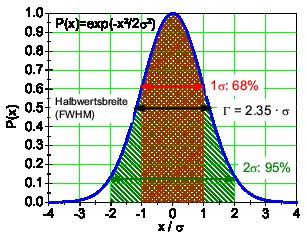
\includegraphics[width=8cm]{00_einl/gaussfkt}
% \end{captionbeside}
 \caption[Gau"ssche Glockenkurve]{\label{a:glockenkurve}Schematische Darstellung
   der Glockenkurve. Die Abzisse ist in Vielfachen von $\sigma$ angegeben.
   Auf die Normierung
   der Ordinate wurde der "Ubersicht wegen verzichtet. Die schraffierten
   Intervalle geben die jeweiligen Sicherheitsintervalle von 68.3~\%
   ($1\sigma$) und 95~\% ($2\sigma$) wieder (siehe Text).}
\end{figure}
%
Weiter kann folgende Formel hergeleitet werden:
%
\begin{equation} \label{i}
 s^2 = \int_{-\infty}^{+\infty}\,P(x) \cdot (x-\bar{x})^{2} dx = \sigma^{2}
\end{equation}
%
Das bedeutet, dass der Parameter $\sigma$ der Glockenkurve mit deren 
Standardabweichung $s$ "ubereinstimmt. Man kann
ferner zeigen, dass die Wahrscheinlichkeit, den wahren Wert
innerhalb des $1\sigma$"=Intervalls um $\bar{x}$ zu finden

\begin{equation} \label{j}
  W(\sigma) = \int_{\bar{x}-\sigma}^{\bar{x}+\sigma} \, P(x) dx =
  0.68
\end{equation}
%
betr"agt. Beziehung (\ref{j}) beinhaltet, dass die Angabe des
mittleren quadratischen Fehlers nicht bedeutet, dass f"ur alle
Messwerte $M_i$ die Abweichung vom Bestwert $M_B$ kleiner als
$\sigma$ ist. Vielmehr betr"agt die relative H"aufigkeit
(Wahrscheinlichkeit oder Sicherheit) hierf"ur nur 68\%.


\subsection{Der Bestwert einer Funktion und Fehlerfortpflanzung}

Der Bestwert einer Funktion $f(x,y,...)$ von verschiedenen
unabh"angigen Messgr"o"sen $x,y,...$ erschwert die Fehlerrechnung
etwas, und es muss das
Fehlerfortpflanzungsgesetz\index{Fehlerfortpflanzungsgesetz}
angewandt werden. Gegeben seien die Messwerte
%
\begin{equation} \label{l}
  x_{i},\quad i=1\ldots r; \hspace{2cm} y_{k},\quad k=1\ldots s \,
  ,
\end{equation}
%
aus denen ein Endergebnis $f_{i,k}=f(x_{i},y_{k})$ berechnet wird.
Beispiel: Berechnung der Fl"ache $A$ eines Rechtecks aus den
Kantenl"angen $x$ und $y$. Es l"asst sich zeigen, dass der Bestwert
$\bar A$ von $A$ gegeben ist durch
%
\begin{equation} \label{m}
 \bar f \equiv  \frac{1}{r} \cdot \frac{1}{s} \cdot
  \sum_{i=1}^{r} \sum_{k=1}^{s} f(x_{i},y_{k}) = f(\bar x, \bar y)
  \, .
\end{equation}
%
Dieses Ergebnis gilt f"ur beliebige Funktionen und beliebig viele
Variablen. Wir bezeichnen jetzt die mittleren quadratischen Fehler
von $f$, $x$ und $y$ mit $\sigma_f$, $\sigma_x$ bzw. $\sigma_y$.
Dann l"asst sich unter Benutzung der Definitionen der mittleren
quadratischen Fehler dieser drei Gr"o"sen zeigen, dass ein
Fehlerfortpflanzungsgesetz\index{Fehlerfortpflanzung} in der Form
%
\begin{equation} \label{n}
 \sigma_{f} =
   \sqrt{\sigma_{x}^{2} \left( \frac{\partial f}{\partial x} \right)^{2}
    +
         \sigma_{y}^{2} \left( \frac{\partial f}{\partial y} \right)^{2}
   }
\end{equation}
%
gilt\footnote{Die gilt, wie eingangs angenommen, {\it nur} f"ur unab"angige
Messgr"o"sen. Andernfalls muss ein zus"atzlicher Term, der die Korrelation
zwischen $x$ und $y$ ber"ucksichtig, hinzugef"ugt werden.}. 
Auch in (\ref{n}) sind beliebig viele Variablen zugelassen.
Spezialf"alle von (\ref{n}) sind:
%
\begin{equation} \label{o}
  \bar f = \bar x + \bar y \qquad \mbox{mit: } \qquad
  \sigma_{f} = \sqrt{\sigma_{x}^{2} + \sigma_{y}^{2}}
\end{equation}
%
\begin{equation} \label{q}
  \bar f = \bar x \cdot \bar y \qquad \mbox{mit: } \qquad
  \frac{\sigma_{f}}{\bar f}  = \sqrt{\left(\frac{\sigma_{x}}{\bar
 x}\right)^{2} + \left(\frac{\sigma_{y}}{\bar y}\right)^{2}} \, .
\end{equation}
%
%


\subsection{Der mittlere quadratische Fehler des Bestwertes}

Die Beziehung (\ref{f}) gibt den mittleren quadratischen Fehler
$\Delta M_{i}$ der Einzelmessung $M_{i}$ an.\footnote{Hier werden
h"aufig auch die Begriffe "`Standardabweichung"' $s$ oder
"`Varianz"' $s^2$ verwendet. Die Verwendung der Begriffe erfolgt
nicht immer einheitlich, man sollte daher auf die jeweilige
Definition achten.} Da aber nicht die Einzelmessung sondern der
Bestwert $M_B$ das Endergebnis darstellt, muss der Fehler des
Bestwertes\index{Fehler!des Mittelwertes} $\Delta M_{B}$ bestimmt
werden. Dazu fassen wir $M_B$ als Funktion der Gr"o"sen $M_{i}$ auf,
d.h.:
%
\begin{equation} \label{s}
M_{B} = \frac{1}{n} \sum_{i=1}^{n}\,M_{i} = f(M_{1}, M_{2},...)
\end{equation}
%
und wenden hierauf das Fehlerfortpflanzungsgesetz
%
\begin{equation} \label{t}
 \Delta M_{B} = \sqrt{\sum_{i=1}^{n}\,\left(\sigma_{i}\,\frac{\partial
 f}{\partial M_{i}}\right)^{2}}
\end{equation}
%
an. Da alle $\sigma_i$ als gleich angenommen werden k"onnen , d.h.
$\sigma_i$ =$\sigma$, und
%
\begin{equation} \label{u}
 \frac{\partial f}{\partial M_{i}} = \frac{1}{n}
\end{equation}
%
ist, ergibt sich schlie"slich:
%
\begin{important}
\begin{equation} \label{v}
 \Delta M_{B} = \frac{\sigma}{\sqrt{n}}  =
  \sqrt{\frac{1}{n(n-1)} \sum_{i=1}^{n} (\Delta M_{i})^{2}} \, .
\end{equation}
\end{important}
%
Genau dies sollte auch in den Protokollen zur Fehlerangabe
verwendet werden.




\subsection{Methode der kleinsten Fehlerquadrate (Minimales $\chi^2$)}

Ein h"aufig vorkommendes Problem ist die Anpassung einer glatten
Kurve an eine Folge von Messpunkten, die zur Bestimmung der
Kurvenparameter dienen sollen. Die Anpassung von Funktionen an
Messwerte erfolgt meist nach der Methode der kleinsten Quadrate
(minimales $\chi^2$). Als Beispiel benutzen wir das radioaktive
Zerfallsgesetz:
%
\begin{equation} \label{w}
  N(t)\,=\,N_{0} \exp(-\lambda t) \, ,
\end{equation}
%
welches die Anzahl $N(t)$ der nicht zerfallenen
radioaktiven Kerne als Funktion der Zeit $t$ beschreibt. In
(\ref{w}) ist $N_0$ die Zahl der Kerne zum Zeitpunkt $t=0$ und
$\lambda$ die Zerfallskonstante, die "uber die Beziehung
%
\begin{equation} \label{x}
  \lambda = \frac{\ln 2}{T_{1/2}}
\end{equation}
%
mit der Halbwertszeit $T_{1/2}$ des radioaktiven Materials
(Nuklids) zusammenh"angt. Zur Vereinfachung setzen wir voraus, dass
$N_0$ aus anderen Messungen bekannt ist, so dass nur noch
$T_{1/2}$ zu bestimmen ist. Wir messen $n$ mal die pro Zeiteinheit
stattfindenen Zerf"alle (Aktivit"at) und stellen uns die Aufgabe,
$T_{1/2}$ durch geeignete Anpassung der Funktion~(\ref{w}) an die
Messwerte zu bestimmen. Die Messung liefert
%
\begin{equation} \label{y}
 \mbox{Wertepaare} (N_i, t_i) \, ,
\end{equation}
%
d.h. die zum Zeitpunkt $t_i$ pro Zeiteinheit gemessene Anzahl
$N_i$ radioaktiver Kerne. Die Vorschrift f"ur die Anpassung der
Funktion (\ref{w}) lautet:
%
\begin{equation} \label{z}
  \chi^{2}(T_{1/2}) =
    \sum_{i=1}^{n} \frac{(N_{i}-N(t_{i}))^{2}}{\sigma_{i}^{2}} = \mbox{Minimum} \, .
\end{equation}
%
In (\ref{z}) bedeutet $\sigma_i$ den mittleren quadratischen
Fehler von $N_i$, der nach den Gesetzen der Statistik f"ur
diskrete, z"ahlbare Ereignisse
(Poisson-Statistik\index{Poisson-Statistik}) durch die Beziehung
%
\begin{equation} \label{aa}
  \sigma_i^2 = N_i
\end{equation}
%
gegeben ist. Wir vergleichen in (\ref{z}) also die Abweichung jedes
Messwertes $N_i$ von der gew"ahlten Kurve mit dem Fehler des
Messwertes und minimieren die Summe der mit dem reziproken Fehler
gewichteten Abweichungsquadrate\index{Abweichungsquadrate}.
Ausdr"ucke der Form (\ref{z}) werden allgemein mit $\chi^2$
bezeichnet und beinhalten die Gau"ssche Methode der kleinsten
Quadrate. Die praktische Auswertung der Vorschrift (\ref{z})
erfolgt, indem man $\chi^2$ f"ur eine Anzahl geeignet erscheinender
Werte $T_{1/2}$ berechnet und das Minimum mit Hilfe einer grafischen
Darstellung der Funktion $\chi^2$($T_{1/2}$) bestimmt.